\begin{minipage}[t]{100mm}
\vspace{3mm}
\section*{Madandmeldelse -- DSB-kaffe}
\fcolorbox{black}{white}{$10^{-6}$ af $\aleph_0$ chokoladekiks}
\vspace{2mm}

Jeg havde glædet mig til at skifte til IC-toget hele vejen siden at være gået i land efter en svømmetur i Smålandsfarvandet og lige havde nået bumletoget fra Bandholm station. Efter flere timers togtur mellem kålmarker, ville jeg nu endelig få dagens første kaffe. Efter uden succes at have lyttet til højtaleren i toget, gik jeg ud at søge efter salgsvognen. Det viste sig at denne i dagens anledning kun tog imod svenske $50$ øre mønter, som dog kunne fremskaffes ved en kort opringning til Gefion, som dog havde tømmermænd og derfor ikke tog det særlig pænt. Efter at have betalt mere end en husalfs årsløn (plus moms) for kaffeen, blev den serveret i et papbæger, varmt nok til at man brændte alle finge (og en tå) inden det første tår kunne tages. Derimod viste kaffen sig at være koldt, så snart den ankom i munden, mindende om noget man finder i kotorets kaffemaskine tidligt mandag morgen efter en forlænget weekend. Ordet kaffe, var dog heller ikke passende, da væsken nok aldrig havde mødt noget der mindede om kaffebønder, nok mindre end de fleste kaffeerstatninger fra krigens tid, heriblandt vand tilsat lidt muld. Jeg drak dog hele koppen, ofrende mit velvære for avisens kvalitet og overlevede dog, hjulpet på vej af i forvejen manglende livslyst. Vågen blev jeg dog, måske mere som en overlevelsesreaktion end som følge af kaffens koffein.

\section*{Parringsritual -- Ewok}
To ewok mødes i skoven, efter at have observeret hinanden i flere dage, begynder de at danse vildt rundt om hinanden, indtil de tilnærmer sig hverandre og ager den andes pels. Efter endnu en omgang dans, omkring det improvisere lejrbål, enedes de om at forplante sig. Inden afslutningen af denne akt, dræbes de begge af en gruppe shockstyrker, som dræber dem og deres for nyligt undfangne afkom.

\begin{center}
%$\quad$\hspace{4cm}
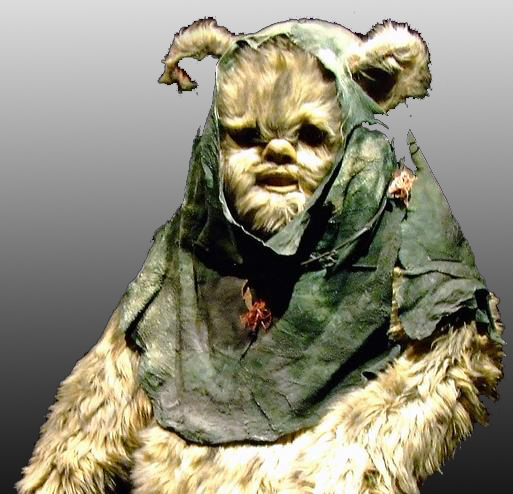
\includegraphics[width=0.8\linewidth]{Ewok.jpg}

\tiny Andreas Rueda Lopez, \url{http://upload.wikimedia.org/wikipedia/commons/b/b1/Ewok_SWExhibition.jpg}, CC-BY-2.0
\end{center}

\end{minipage}
